\subsection{Revised source and frozen diagnostics on unused catalogue values}
\label{sec:he0435-revised-results}
The development selection retains candidate 1 with a regular compact matter component of \(1.000\times10^{8}\)\,$M_\odot$ and scale 0.03\,kpc.
The conventional and conditional R1 applications have 5 and 5 verified stationary images, respectively; all additional images enter the summed central-light constraint.
The nearly degenerate development objectives do not measure a nuclear mass. The selected positive component is a conditional matter surrogate, not an inferred black hole or a solved stellar equation of state.

The original scalar and metric equations are applied to the total enclosed matter once:
\[ Cx^2p-\frac{4}{\widehat\lambda}xp^2=-\widehat b\,m(x),\qquad 2x^2\frac{d\Phi}{dx}+\widehat b x^2p=2m(x). \]
Here $x=rH_0$, $m(x)=GM(<r)H_0$, $\widehat b=b_T/M_{\rm Pl}$, $p=\pi_T^{\prime}/(M_{\rm Pl}H_0)$ and $c=1$, with the previously fixed $\widehat\lambda=\lambda/(M_{\rm Pl}H_0^2)$.
At $r=0.03$\,kpc, the computed section has $\widehat\rho=\rho/(M_{\rm Pl}^2H_0^2)$ equal to \(3.734\times10^{9}\), reduced source $\widehat J_{\rm eff}=J_{\rm eff}/(M_{\rm Pl}H_0^2)=-\widehat b\widehat\rho/2$ equal to \(-1.712\times10^{8}\), and $p$ equal to \(-3.599\times10^{-5}\).
The scalar integrated left side and source are \(-3.495\times10^{-17}\) and \(-3.495\times10^{-17}\), while the metric Gauss left side and source are \(7.623\times10^{-16}\) and \(7.623\times10^{-16}\).
Across the evaluated sections the maximum relative scalar and Gauss residuals are \(3.419\times10^{-16}\) and \(2.168\times10^{-16}\).
Activating R1 on the fixed conventional body, source, maps and clock gives B/C/D-minus-A delay offsets $(20.60284,1.00422,31.21607)$\,s and a maximum coordinate image displacement \(2.075\times10^{1}\)\,$\mu$as. Separately refitted model predictions below need not retain those fixed-reference offsets.

The compact-source model's LCO test opens 162 previously unused A/B/D measurements, conditional on 54 allowed C measurements from the same later LCO epochs. The no-driver secondary forecast opens all 216 measurements. No brightness, delay, offset, calibration or source parameter is refitted to these target values. These scores belong to this frozen geometry, preceding the explicit G1 revision below.
Table~\ref{tab:he0435-revised-primary} reports the normalized joint conditional density and marginal predictive diagnostics. The joint log density is a density in the declared magnitude units; epochs are correlated, and its value is not a chi-square significance or an independent-event count.
\begin{table}[t]
\caption{Frozen compact-source models on unused LCO R A/B/D observations, with image C as the allowed driver. Coverage is the empirical fraction within marginal 95\% mixture intervals; width and the proper 95\% interval score are in magnitudes. Larger joint log density and smaller interval score are preferred.}\label{tab:he0435-revised-primary}
\centering\footnotesize
\begin{tabular}{lrrrrr}\toprule
Model & Joint $\log p$ & RMSE & \shortstack{95\%\\coverage} & Width & \shortstack{95\%\\interval score}\\\midrule
Empirical delay ensemble & 292.467 & 0.0780 & 98.77 & 0.6566 & 0.6640\\
Conventional macro & 291.071 & 0.0772 & 98.77 & 0.6699 & 0.6779\\
Conditional R1 macro & 291.071 & 0.0772 & 98.77 & 0.6699 & 0.6779\\
Fixed-body R1 activation & 291.071 & 0.0772 & 98.77 & 0.6699 & 0.6779\\
Zero-delay control & 289.016 & 0.0795 & 98.77 & 0.6245 & 0.6334\\
\bottomrule\end{tabular}
\end{table}

The old undercoverage is not reproduced in this unused-catalogue batch, but the revised uncertainty is conservative rather than sharply calibrated: nominal 68.27\% intervals contain 94.44\% of primary targets, and image B has mean 95\% width 1.3014\,mag. The no-driver secondary forecast retains mean signed residual +0.1761\,mag. Moreover, the zero-delay control has mean 95\% interval score 0.6334\,mag, compared with 0.6779\,mag for conventional, while conventional has the larger joint log density. Coverage, width, bias and the different proper scores must therefore be considered together; no uniformly superior model or precise delay recovery is established by this batch.
The conventional intervals contain 160 of 162 primary targets (98.77\%). The conditional R1-minus-conventional joint log-score difference is \(-3.460\times10^{-5}\); this is a finite-model predictive comparison, not a Bayes factor from a completed physical-state posterior.
The fixed-body R1 activation has a primary log-score difference of \(1.507\times10^{-4}\) relative to conventional, with the same optical nuisance parameters. It isolates the original scalar response; the separately refitted R1 comparison also includes development nuisance and optimizer movement and cannot be attributed entirely to that activation.
The matched conventional effective-mass representation has the same retained optical transfer as conditional R1 and therefore the same score by construction; it is not an independent confirmation.
\begin{table}[t]
\caption{Image-resolved primary diagnostics. Each image contributes 54 unused observations. These are correlated marginal diagnostics, not 54 independent coverage trials.}\label{tab:he0435-revised-images}
\centering\small\begin{tabular}{lrrr|rrr}\toprule
&\multicolumn{3}{c}{Conventional}&\multicolumn{3}{c}{Conditional R1}\\
Image & RMSE & Coverage (\%) & Width & RMSE & Coverage (\%) & Width\\\midrule
A & 0.0489 & 96.30 & 0.3667 & 0.0489 & 96.30 & 0.3667\\
B & 0.1192 & 100.00 & 1.3014 & 0.1192 & 100.00 & 1.3014\\
D & 0.0361 & 100.00 & 0.3417 & 0.0361 & 100.00 & 0.3417\\
\bottomrule\end{tabular}
\end{table}

Without the C driver, the conventional all-image forecast has joint log density 390.118, RMSE 0.2170\,mag, 95\% coverage 100.00\%, mean interval width 1.2534\,mag and mean interval score 1.2534\,mag. The secondary R1-minus-conventional log-score difference is \(2.497\times10^{-6}\). Primary and secondary targets overlap and cannot be counted as separate confirmations.
\begin{figure}[t]
\centering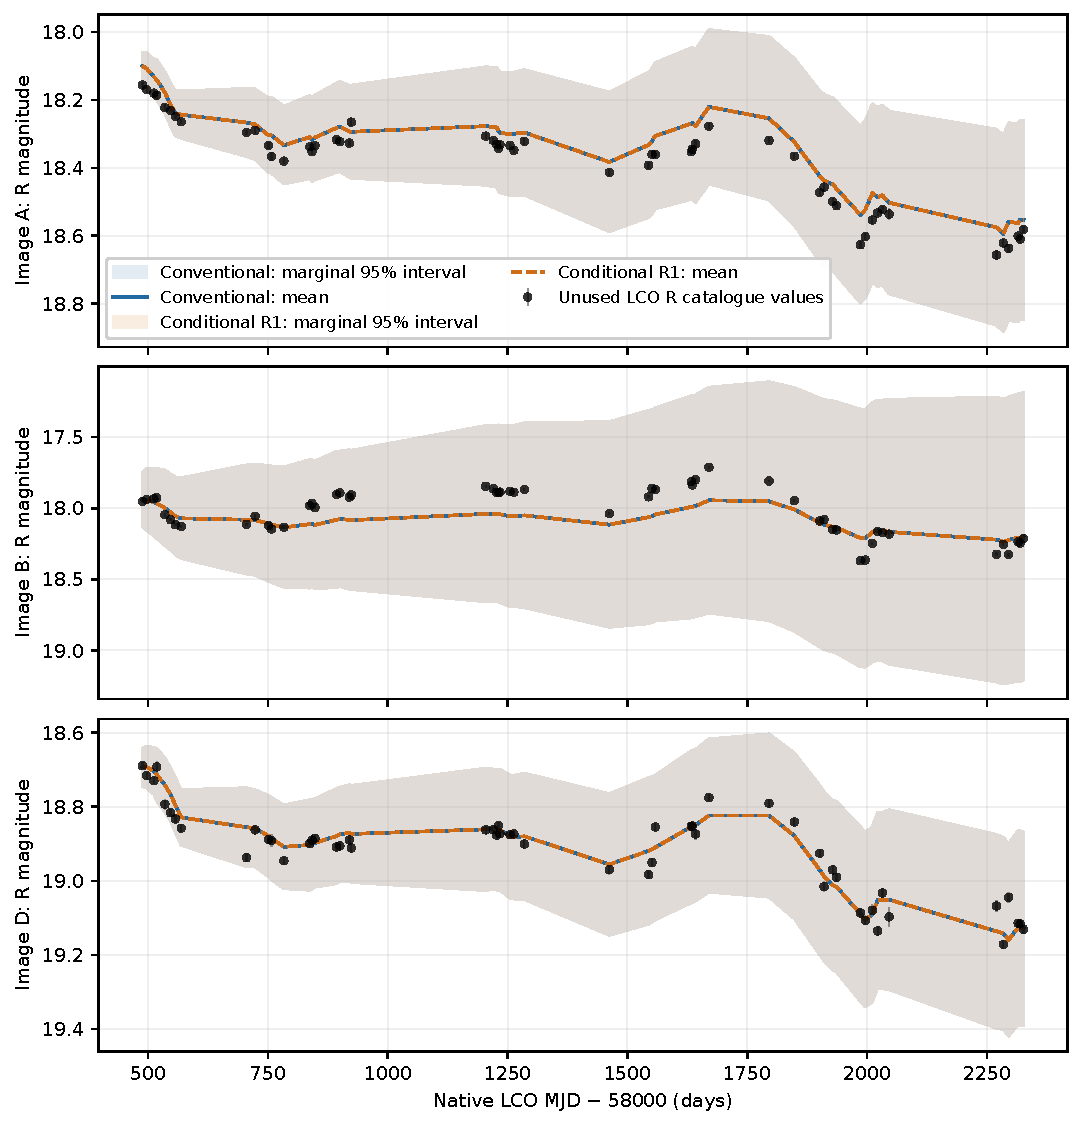
\includegraphics[width=\textwidth]{figures/he0435_revision_unused_prediction.pdf}
\caption{Unused LCO R observations and the frozen C-driven conventional and conditional R1 predictions. Shading shows marginal 95\% mixture intervals, including the development-only image calibration. The curves and bands can nearly coincide. Straight segments join predictions only at observed epochs and are not an additional fitted variability curve.}\label{fig:he0435-revised-unused}
\end{figure}

The experiment tests a fixed, calibrated finite nuisance ensemble. Its short chains have maximum basic $\widehat R=5.19$, so the mixture is not a demonstrated converged posterior and supplies no complete physical-state marginalization. These LCO catalogue values were unused in model selection and arise from a separate monitoring campaign. Their retrospective difference-imaging reference includes 2022 data, however, so photon-disjoint calibration and validation are not established. Common reduction errors and prior qualitative publication awareness limit blinding. The central-image HST result is conditional on the empirical PSFs, adopted marginal noise and macro-to-observed flux relation. These qualifications, and any remaining undercoverage in the actual test, remain part of the result. Neither the statistical ensemble nor a close conventional/R1 score establishes a unique envelope state or a BHSM detection; the physical guard remains $2\times10^{-10}$ and no physical admission is asserted.
